\chapter{Influence Diagrams}
\label{ch-influ-diag}

This chapter is based on Refs.\cite{sha-influ-diag}
and \cite{limid-one}.


An {\bf Influence Diagram (ID)} is
a DAG that generalizes a bnet by adding
2 new types of nodes. IDs have 3 types of nodes: chance, decision and value nodes, represented, respectively, by ovals, squares and diamonds. Table \ref{tab-id-nodes} compares these 3 types of nodes.

% Please add the following required packages to your document preamble:
% \usepackage[table,xcdraw]{xcolor}
% Beamer presentation requires \usepackage{colortbl} instead of \usepackage[table,xcdraw]{xcolor}
\begin{table}[h!]
\begin{tabular}{|l|l|l|l|}
\hline
                                                                                            & \cellcolor[HTML]{FFFFC7}\begin{tabular}[c]{@{}l@{}}Chance node \\ (oval)\end{tabular} & \cellcolor[HTML]{FFFFC7}\begin{tabular}[c]{@{}l@{}}Decision node\\ (square)\end{tabular} & \cellcolor[HTML]{FFFFC7}\begin{tabular}[c]{@{}l@{}}Value node\\ (diamond)\end{tabular} \\ \hline
\cellcolor[HTML]{FFFFC7}type of states                                                      & discrete                                                                     & discrete, binary usually                                                                       & continuous                                                                             \\ \hline
\cellcolor[HTML]{FFFFC7} deterministic?                                                   & Not in general                                                                        & Yes                                                                                      & Yes                                                                                    \\ \hline
\cellcolor[HTML]{FFFFC7}transition info\footnote{by ``transition info" of a node, we
mean ``personal" node info
other than a list of the states of the node and a list 
of its parent nodes}                                                    & TPM                                                                                   & 
deterministic TPM                                                                                 & utility function                                                                       \\ \hline
\cellcolor[HTML]{FFFFC7}children type                                                       & chance, decision, value                                                               & chance, decision, value                                                                  & None                                                                                   \\ \hline
\cellcolor[HTML]{FFFFC7}\begin{tabular}[c]{@{}l@{}}can be fixed\\ by observer?\end{tabular} & Yes                                                                                   & Yes                                                                                      & No                                                                                     \\ \hline
\end{tabular}
\caption{Comparison of the 3 types
of nodes in an influence diagram.
The only difference between Chance and 
Decision nodes is that Chance nodes have
a probabilistic TPM and Decision nodes have
a deterministic one.}
\label{tab-id-nodes}
\end{table}
Let

$\rvc.=$ set of {\bf chance nodes}

$\rvd.=$ set of {\bf decision nodes}
Assume $\rvd_i$ are in chronological
order, i.e., $\rvd_i$ occurs before $\rvd_{i+1}$ for all $i$.

$\rvu.=$ set of {\bf utility nodes}. Often, utility nodes are called {\bf value nodes} and only their sum is called a utility node.

$\rvx.= \rvc. \cup \rvd. \cup \rvu.$ all nodes

$\rve.=$ {\bf evidence nodes}, the subset of the chance nodes $\rvc.$ that is {\bf apriori observed}
(i.e. measured before the experiment starts). If a decision node has a 
chance node as a parent,
we will assume it is measured immediately before the decision is made,
not apriori.


$u_i(pa(\rvu_i))=$ {\bf partial utility function}

$u(\rvc., d.)=\sum_i u_i(pa(\rvu_i))$ {\bf total utility function }

\begin{itemize}


\item{\bf Optimal Strategy}

Let
\beq
L_i = \lim_{pa(d_i)\rarrow pa( d_i)^*}
\eeq
for $i=1,2, \ldots, nd$.
Note that



\beq
pa(d_1)^* = \argmax_{pa(d_1)}E_{\rvc.-pa(\rvd_1)}[u(\rvc., d.)]
\eeq


\beq 
pa(d_2)^* = \argmax_{d_2}L_1E_{\rvc.-pa(\rvd_1)-pa(\rvd_2)}[u(\rvc., d.)]
\eeq

\beq 
pa(d_3)^* = \argmax_{d_3}L_2 L_1 E_{\rvc.-pa(\rvd_1)-pa(\rvd_2)-pa(\rvd_3)}[u(\rvc., d.)]
\eeq

\beq
d_i^* = d_i(pa(d_i)^*)
\eeq


\item {\bf Expected Utility}
\beq
EU(d.)=E_{\rvc.}[u(\rvc., d.)]=
\sum_{c.} P(c.)u(c., d.)
\eeq
where 
\beq
P(c.)= P(c.-e.)\delta(e., e.')
\eeq
or
\beq
P(c.)= P(c.-e.-y.)\delta(e., e.')\delta(y., y^*)
\eeq
where 
\beq 
y^*.= \cup_{i=1}^{nd}pa(d_i)^*
\eeq


\item {\bf Maximum Expected Utility}

\beq
MEU=EU(d.^*)
\eeq
where $d.^*$ is the optimal strategy.


\item {\bf Limited Memory ID (LIMID)}. 

LIMIDs were first introduced 
in Ref.\cite{limid-one}. According to that reference, LIMIDs are ``multistage decision problems in which the traditional assumption of no forgetting is
relaxed." 
Note that ``multistage bnet" is another term
for a dynamic bnet (see Chapter \ref{ch-dyn-bnets}).
Figs.\ref{fig-pre-limid} and \ref{fig-post-limid}
come from Ref.\cite{limid-one} and describe pig farming
at various times $T=\{1,2,3,4\}$.

Node $\rvh_i\in\bool$
refers to the health of a pig at time $i$.

Node $\rvt_i\in \bool$ refers to a test 
conducted on the pig at time $i$.

Node $\rvd_i\in \bool$ refers to a decision 
made by the farmer at time $i$ on whether to medicate the pig.

Node $\rvu_i\in \bool$ refers to the utility (monetary value)  
of medicating the pig at time $i$.

 
Fig.\ref{fig-pre-limid} shows a dynamic bnet that
obeys the {\bf no forgetting} assumption so every decision is
privy to the state of all previous decision and chance nodes.
Fig.\ref{fig-post-limid} shows the same bnet as 
Fig.\ref{fig-pre-limid} after all arrows entering a decision $\rvd_i$ and originating at an earlier time, have been removed.



\begin{figure}[h!]
\centering
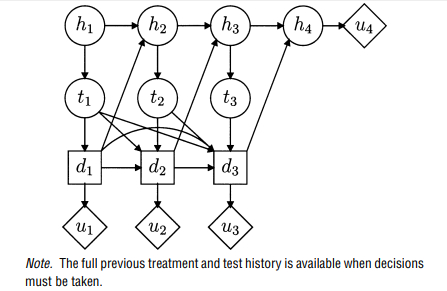
\includegraphics[width=4in]
{influ-diag/pre-limid.jpg}
\caption{Pig farming ID that obeys the ``no-forgetting"
assumption.  
}
\label{fig-pre-limid}
\end{figure}


\begin{figure}[h!]
\centering
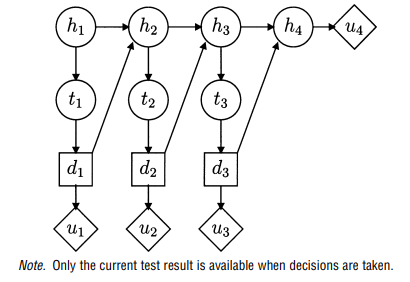
\includegraphics[width=4in]
{influ-diag/post-limid.jpg}
\caption{Pig farming ID that obeys the  LIMID
assumption. This ID is the same as the ID of Fig.\ref{fig-pre-limid},
except that the arrows pointing to a decision and originating at a previous time, have been removed.}
\label{fig-post-limid}
\end{figure}

\item {\bf Finding optimal strategy }

Ref.\cite{sha-influ-diag} proposes 3 exact methods for
finding the optimal strategy, EU and MEU.
1) conversion to a decision
tree 2) evaluation directly as influence diagrams
3) conversion to a rooted cluster tree.
We will only discuss exact method 1
and use as an example,
the ID shown in Fig.\ref{fig-sha-fig1} 
which comes from Ref.\cite{sha-influ-diag}.


\begin{figure}[h!]
\centering
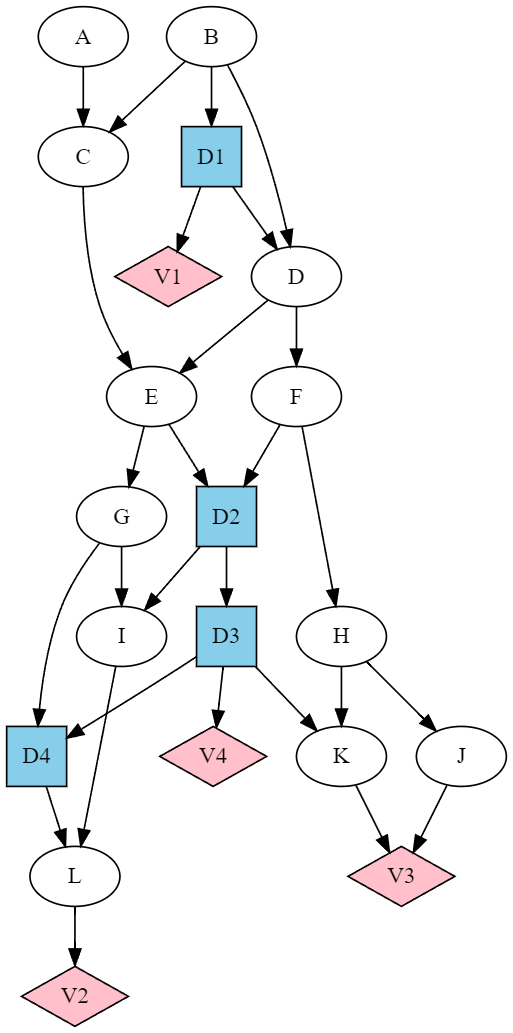
\includegraphics[width=2.3in]{influ-diag/sha-fig1.png}
\caption{Example of ID from Ref.\cite{sha-influ-diag}}
\label{fig-sha-fig1}
\end{figure}


\begin{figure}[h!]
\centering
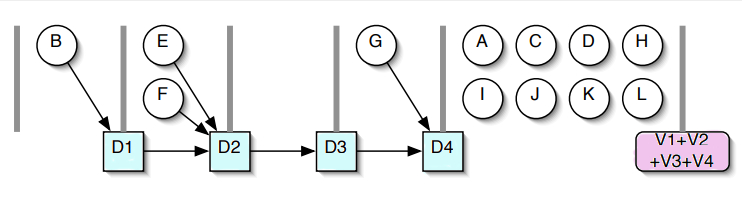
\includegraphics[width=6in]
{influ-diag/influ-diag-stages.jpg}
\caption{Different decision stages for the ID of Fig.\ref{fig-sha-fig1}}
\label{fig-jensen-stages}
\end{figure}

\begin{figure}[h!]
\centering
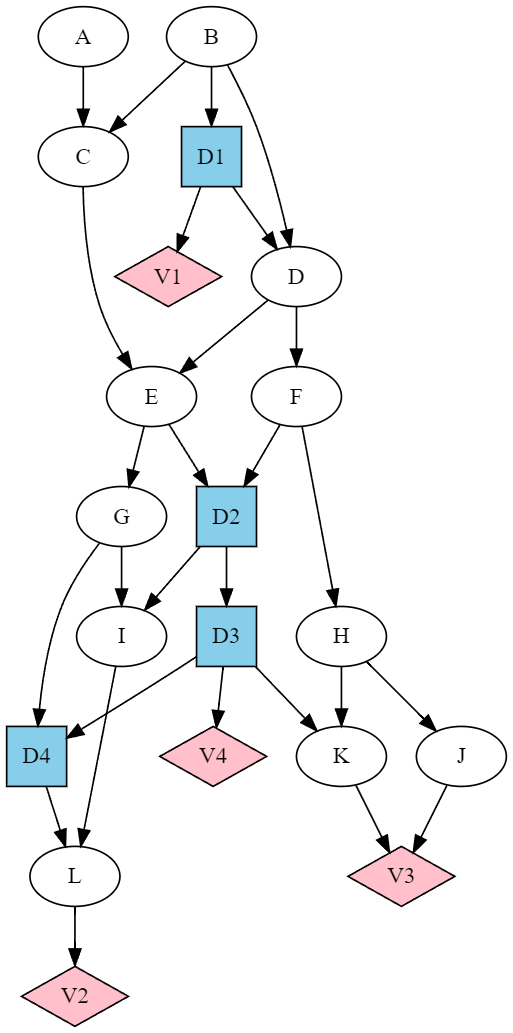
\includegraphics[width=2.3in]{influ-diag/sha-fig1.png}
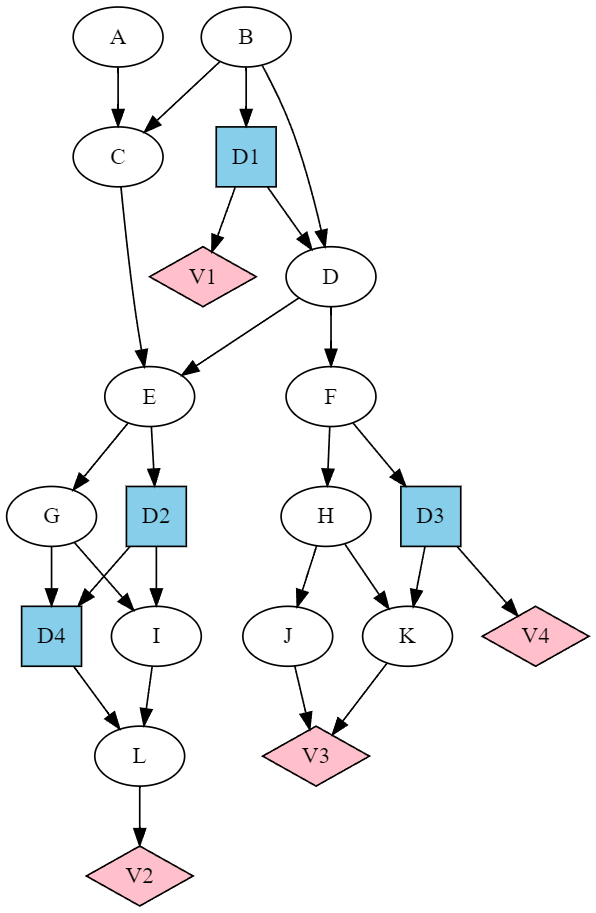
\includegraphics[width=2.3in]{influ-diag/sha-fig3.png}
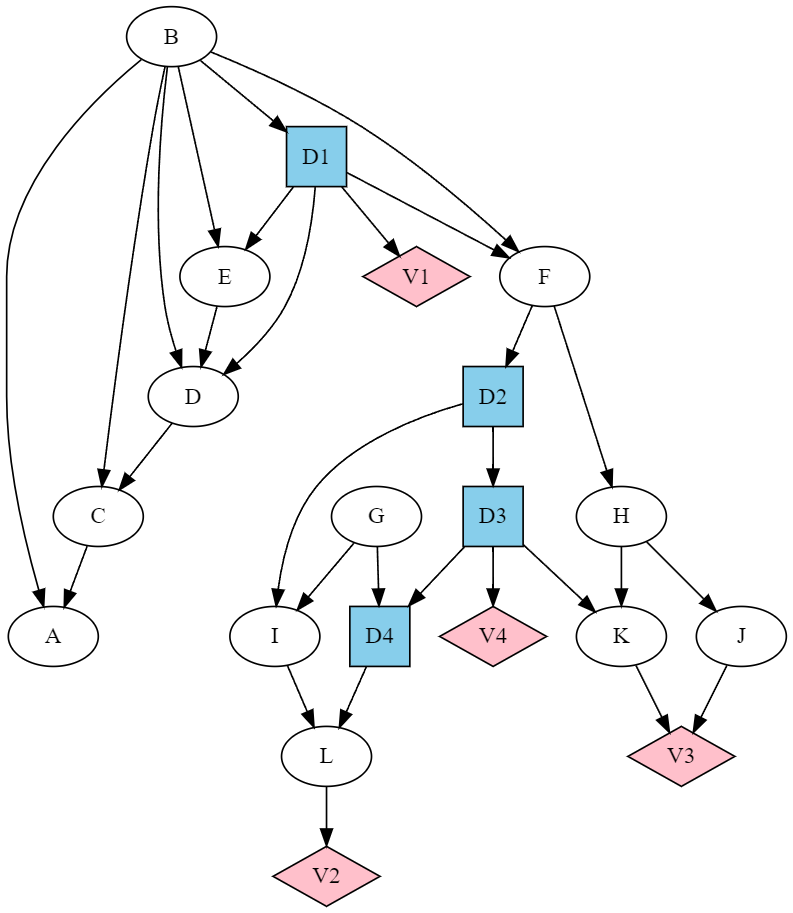
\includegraphics[width=3in]{influ-diag/sha-fig4.png}
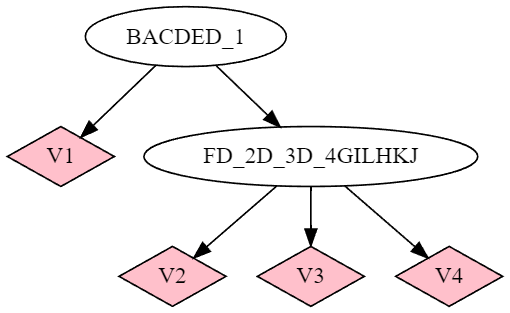
\includegraphics[width=2in]{influ-diag/sha-fig4coarse.png}
\caption{T=Top, B=Bottom, L=Left, R=Right. {\bf TL:} the ID of Fig.\ref{fig-sha-fig1},
{\bf TR:} the ID of TL after reduction to requisite
observations. {\bf BL:} the ID of TL after reduction to a tree.
{\bf BR:} the ID of TR after merging some nodes.}
\label{fig-sha-fig134}
\end{figure}





\end{itemize}